\documentclass[tikz, border=2pt]{standalone}
\usepackage{amsmath}

\begin{document}
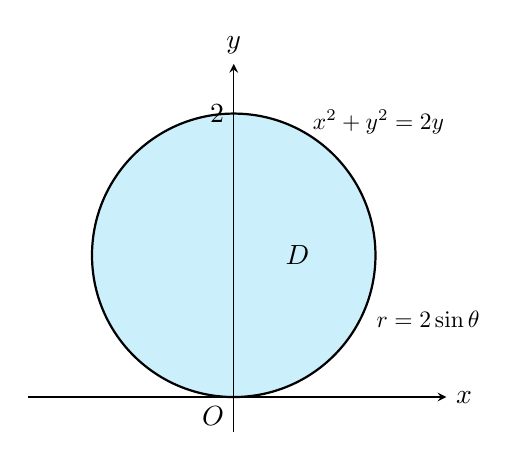
\begin{tikzpicture}[scale=1.8, >=stealth]
    % D: x^2+y^2 <= 2y, a unit circle centered at (0,1).
    \fill[cyan!20] (0,1) circle (1);

    \draw[->] (-1.45,0) -- (1.5,0) node[right] {$x$};
    \draw[->] (0,-0.25) -- (0,2.35) node[above] {$y$};

    \draw[thick] (0,1) circle (1);
    \draw[dashed] (0,0) -- (0,2) node[left] {$2$};

    \node[below left] at (0,0) {$O$};
    \node at (0.45,1) {$D$};
    \node[above right, scale=0.85] at (0.5,1.8) {$x^2+y^2=2y$};
    \node[right, scale=0.85] at (0.95,0.55) {$r=2\sin\theta$};
\end{tikzpicture}
\end{document}
